\documentclass{article}
\usepackage{amsfonts, amsmath, amssymb, amsthm} % Math notations imported
\usepackage{enumitem}
\usepackage{graphicx}
\usepackage{setspace}
\usepackage{indentfirst}
\usepackage[margin=1in]{geometry}
\graphicspath{{./images/}} % Path to images

% \begin{figure}[htb!]
%      \centering
%      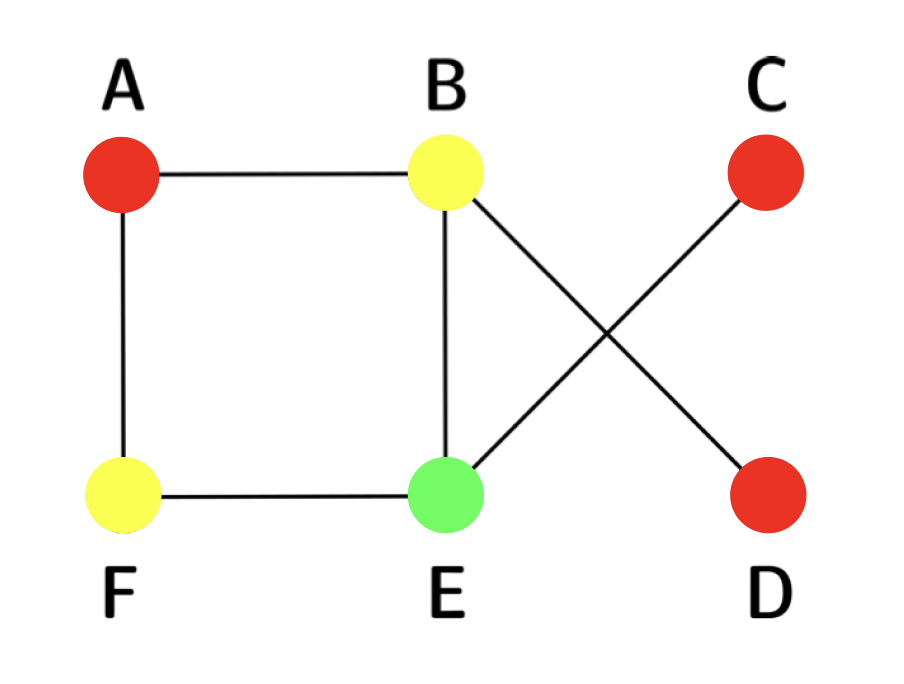
\includegraphics[scale=0.5]{coloring.png}
%      \caption{Coloring of the graph.}
% \end{figure}

% \begin{figure}[htb]
%     \qquad
%     \begin{minipage}{.4\textwidth}
%         \centering
%         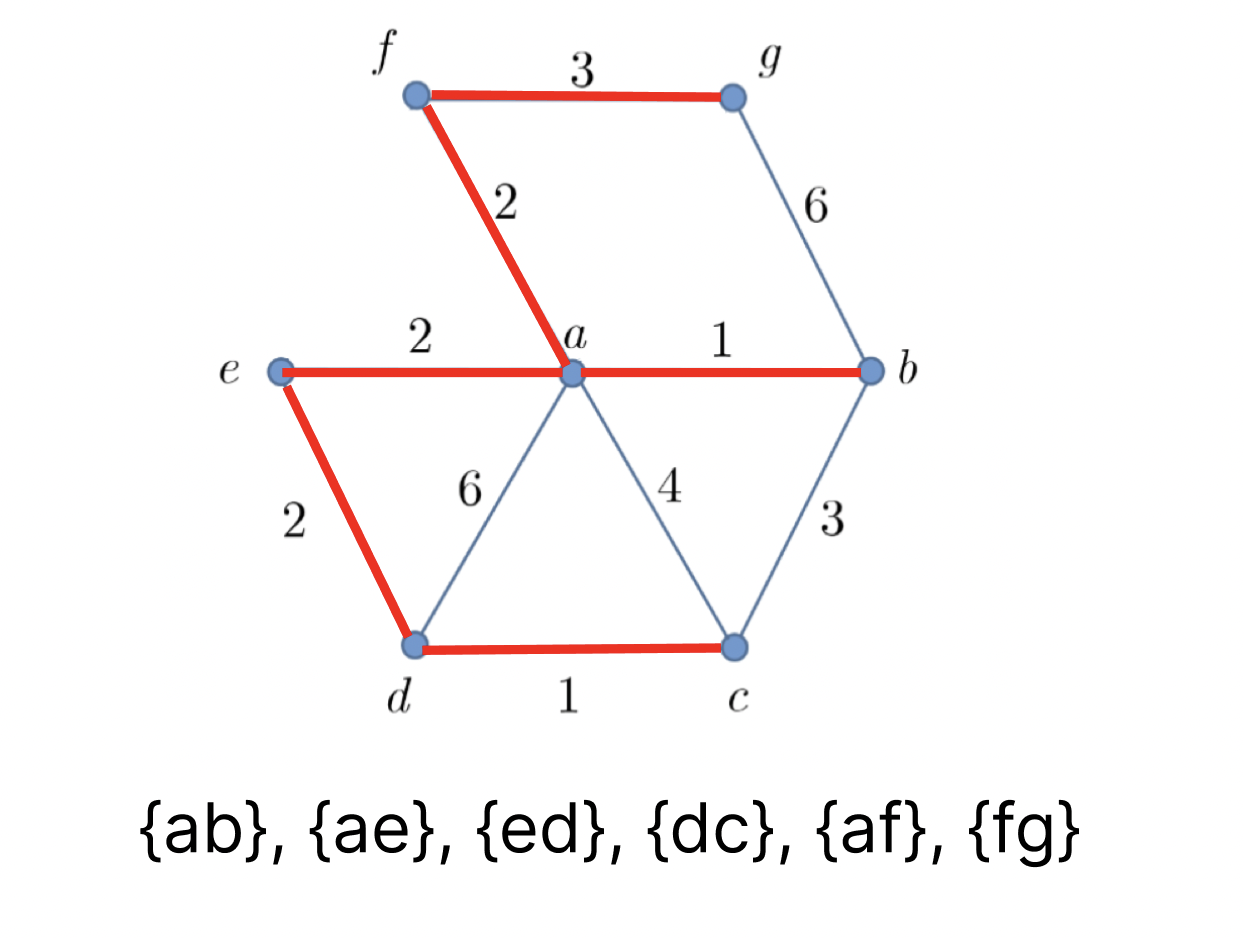
\includegraphics[scale=0.35]{prims.png}
%         \caption{}
%     \end{minipage}    
%     \qquad
%     \begin{minipage}{.4\textwidth}
%         \centering
%         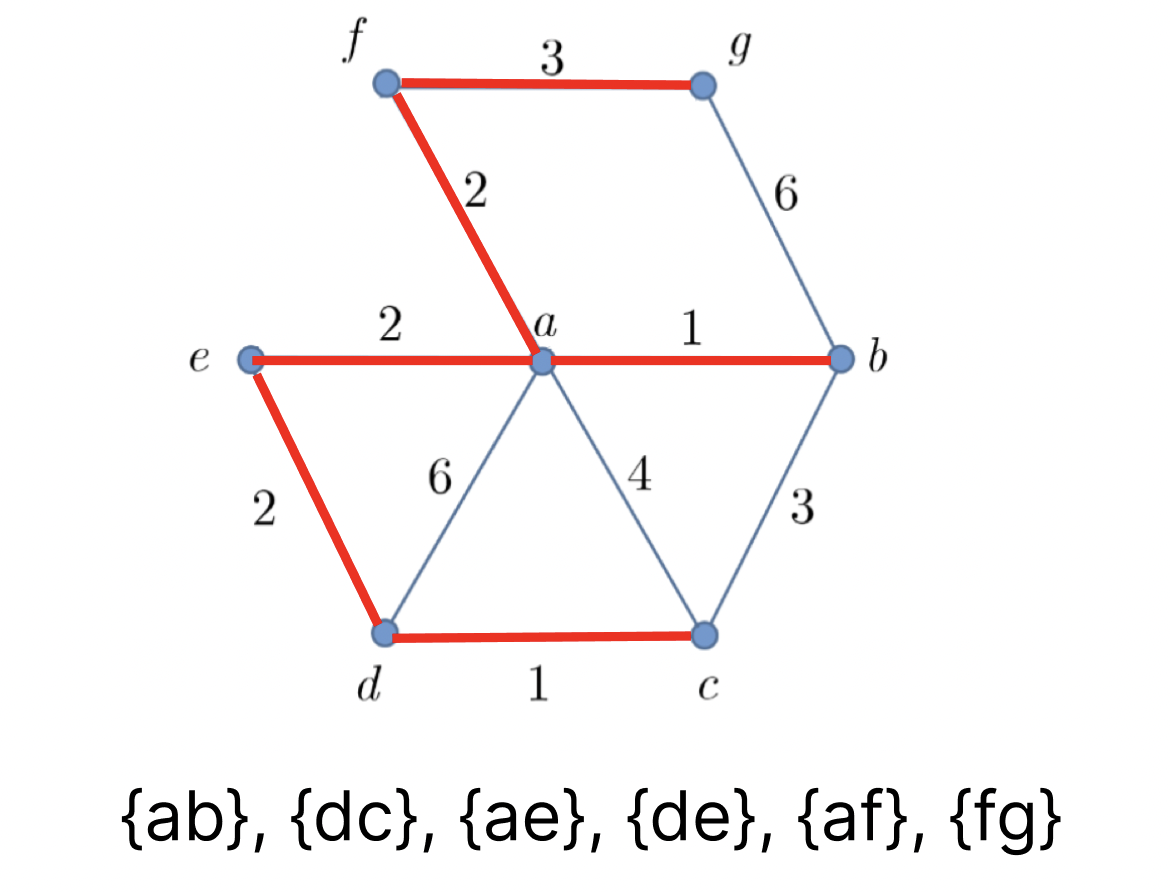
\includegraphics[scale=0.35]{kruskal.png}
%         \caption{}
%     \end{minipage}        
% \end{figure} 

\newtheorem{thm}{Theorem}
\newtheorem{proposition}[thm]{Proposition}
\newtheorem{cor}[thm]{Corollary}

% title information
\title{Math 110 HW4}
\author{Neo Lee}
\date{09/23/2023}

\setstretch{1.15}
% main content
\begin{document} 

% placing title information; comment out if using fancyhdr
\maketitle 

\subsection*{Problem 1.}
Let $a, b\in \mathbb{R}$. Define $T: {\cal P}(\mathbb{R}) \to \mathbb{R}^2$ by
$$ Tp := (2 p(1) + 5 p'(2) +a p(-1) p(3), \int_{-1}^1 x^3 p(x) \, dx + b \sin p(0)). $$
Under what conditions on $a$ and $b$ is the map $T$ linear?

\begin{proof}[Solution]
    We will verify the linearity of $T$ by checking the two properties of linear maps separately on 
    the first and second components of $Tp$.

    \textbf{Additivity of first coordinate:} Let $p, q \in \mathcal{P}(\mathbb{R})$. Then,
    \begin{align*}
        T(p+q)^{(1)} & = 2(p+q)(1) + 5(p+q)'(2) + a(p+q)(-1)(p+q)(3) \\
        & = 2(p(1) + q(1)) + 5(p'(2) + q'(2)) + a(p(-1)+q(-1))(p(3)+q(3)) \\
        & = 2p(1) + 2q(1) + 5p'(2) + 5q'(2) + ap(-1)p(3) + ap(-1)q(3) + aq(-1)p(3) + aq(-1)q(3) \\
        & = 2p(1) + 5p'(2) + ap(-1)p(3) + 2q(1) + 5q'(2) + aq(-1)q(3) + \underline{\left(ap(-1)q(3) + aq(-1)p(3)\right)} \\
        & = Tp^{(1)} + Tq^{(1)} + \underline{a\left(p(-1)q(3) + q(-1)p(3)\right)}.
    \end{align*}

    Hence, the linearity only holds if $a(p(-1)q(3) + q(-1)p(3)) = 0$ for all 
    $p, q \in \mathcal{P}(\mathbb{R})$. This is only possible when $a = 0$ [we can show by 
    considering $p,q$ such that $p(-1)q(3) + q(-1)p(3)\neq 0$].

    \textbf{Additivity of second coordinate:} Let $p, q \in \mathcal{P}(\mathbb{R})$. Then,
    \begin{align*}
        T(p+q)^{(2)} & = \int_{-1}^1 x^3 (p+q)(x) \, dx + b \sin (p+q)(0) \\
        & = \int_{-1}^1 x^3 p(x) \, dx + \int_{-1}^1 x^3 q(x) \, dx + \underline{b \sin p(0) + b \sin q(0)} \\
        & = Tp^{(2)} + Tq^{(2)} + \underline{b \left(\sin p(0) + \sin q(0)\right)}.
    \end{align*}

    Again, the linearity only holds if $b(\sin p(0) + \sin q(0)) = 0$ for all 
    $p, q \in \mathcal{P}(\mathbb{R})$. This is only possible when $b = 0$ [we can show by 
    considering $p,q$ such that $\sin p(0) + \sin q(0)\neq 0$].

    Finally, we check that homogeneity still holds when $a = b = 0$.

    \textbf{Homogeneity of first coordinate:} Let $p \in \mathcal{P}(\mathbb{R})$ and 
    $c \in \mathbb{R}$. Then,
    \begin{align*}
        T(cp)^{(1)} & = 2(cp)(1) + 5(cp)'(2) + 0(cp)(-1)(cp)(3) \\
        & = c\cdot2p(1) + c\cdot5p'(2) + c^2\cdot0p(-1)p(3) \\
        & = c\left(2p(1) + 5p'(2)\right) \\
        & = cTp^{(1)}.
    \end{align*}

    \textbf{Homogeneity of second coordinate:} Let $p \in \mathcal{P}(\mathbb{R})$ and
    $c \in \mathbb{R}$. Then,
    \begin{align*}
        T(cp)^{(2)} & = \int_{-1}^1 x^3 (cp)(x) \, dx + 0 \sin (cp(0)) \\
        & = c\int_{-1}^1 x^3 p(x) \, dx + 0 \\
        & = cTp^{(2)}.
    \end{align*}
\end{proof}

\newpage
\subsection*{Problem 2.}
Suppose $T \in {\cal L} (V,W)$, $v_1, \ldots, v_m \in V$ and the list
$Tv_1, Tv_2, \ldots Tv_m$ spans $W$. Prove or disprove that the list $v_1, \ldots, v_m$ spans $V$. 

\begin{proof}[Solution]
    I will provide a counterexample to show that the statement is false. Let $V = \mathbb{R}^2$,
    $W = \mathbb{R}$, and $T: V \to W$ be defined by $T: (x, y) \rightarrow (x)$. Let $v_1 = (1, 0)$. 
    Then, $Tv_1 = (1)$, which spans $W$. However, $v_1$ does not span $V=\mathbb{R}^2$ obviously.
\end{proof}

\newpage
\subsection*{Problem 3.}
Let $V={\cal P}_2(\mathbb{R})$, $W=\mathbb{R}$. Are the maps $$T_1: f\mapsto f(0), \quad T_2: f\mapsto f'(1), 
\quad T_3 : f\mapsto \int_{0}^1 f(x) dx$$ in ${\cal L}(V,W)$? Are they linearly independent?

\begin{proof}[Solution]
    To check if the maps are linear, we will check whether they satisfy additivity and homogeneity.

    \textbf{Additivity of $T_1$:} Let $f, g \in \mathcal{P}_2(\mathbb{R})$. Then,
    \begin{align*}
        T_1(f+g) & = (f+g)(0) \\
        & = f(0) + g(0) \\
        & = T_1(f) + T_1(g).
    \end{align*}

    \textbf{Homogeneity of $T_1$:} Let $f \in \mathcal{P}_2(\mathbb{R})$ and $c \in \mathbb{R}$. Then,
    \begin{align*}
        T_1(cf) & = (cf)(0) \\
        & = c\cdot f(0) \\
        & = cT_1(f).
    \end{align*}

    \textbf{Additivity of $T_2$:} Let $f, g \in \mathcal{P}_2(\mathbb{R})$. Then,
    \begin{align*}
        T_2(f+g) & = (f+g)'(1) \\
        & = f'(1) + g'(1) \\
        & = T_2(f) + T_2(g).
    \end{align*}

    \textbf{Homogeneity of $T_2$:} Let $f \in \mathcal{P}_2(\mathbb{R})$ and $c \in \mathbb{R}$. Then,
    \begin{align*}
        T_2(cf) & = (cf)'(1) \\
        & = cf'(1) \\
        & = cT_2(f).
    \end{align*}

    \textbf{Additivity of $T_3$:} Let $f, g \in \mathcal{P}_2(\mathbb{R})$. Then,
    \begin{align*}
        T_3(f+g) & = \int_{0}^1 (f+g)(x) dx \\
        & = \int_{0}^1 f(x) + g(x) dx \\
        & = \int_{0}^1 f(x) dx + \int_{0}^1 g(x) dx \\
        & = T_3(f) + T_3(g).
    \end{align*}

    \textbf{Homogeneity of $T_3$:} Let $f \in \mathcal{P}_2(\mathbb{R})$ and $c \in \mathbb{R}$. Then,
    \begin{align*}
        T_3(cf) & = \int_{0}^1 (cf)(x) dx \\
        & = \int_{0}^1 cf(x) dx \\
        & = c\int_{0}^1 f(x) dx \\
        & = cT_3(f).
    \end{align*}

    To check linear independence of $T_1, T_2, T_3$, we will check if the only solution to the equation 
    $$\alpha T_1 + \beta T_2 + \gamma T_3 = 0$$ is $\alpha = \beta = \gamma = 0$.

    Let $f(x) = ax^2 + bx + c$. Then,
    \begin{align*}
        \alpha T_1 + \beta T_2 + \gamma T_3 = \alpha f(0) + \beta f'(1) + \gamma \int_{0}^1 f(x) dx & = 0 \\
        \alpha c + \beta (2a + b) + \gamma \left(\frac{a}{3} + \frac{b}{2} + c\right) & = 0 \\
        6\alpha c + 12\beta a + 6\beta b + 2\gamma a + 3\gamma b + 6\gamma c & = 0 \\
        (12\beta + 2\gamma)a + (6\beta + 3\gamma)b + (6\alpha + 6\gamma)c & = 0.
    \end{align*}
    We claim this is only true for all $a, b, c \in \mathbb{R}$ if 
    $$\begin{cases}
        12\beta + 2\gamma = 0 \\
        6\beta + 3\gamma = 0 \\
        6\alpha + 6\gamma = 0.
    \end{cases}$$
    \underline{Proof sketch of the claim:} Assume without loss of generality that 
    $12\beta + 2\gamma \neq 0$ is part of the solution. Then, take $a' = 2a$, and we will reach a 
    contradiction that the equation does not equal to 0.

    Now we can solve the system of equations by gaussian elimination, and we will get 
    $\alpha = \beta = \gamma = 0$. Hence, the maps are linearly independent.
\end{proof}

\newpage
\subsection*{Problem 4.}
Suppose $V$ is a vector space and $S$, $T \in {\cal L}(V,V)$ are such that
$$  {\rm range} \, S \subset {\rm null}\, T.$$
Prove or disprove that $ST=TS=0$.

\begin{proof}[Solution]
    We will provide a counter example.

    Consider $V = \mathbb{R}^3$. Define 
    $$T: (x,y,z) \rightarrow (x, 0, 0)$$
    $$S: (x,y,z) \rightarrow (0, 0, x).$$
    It is trivial to see that $S, T$ are indeed linear maps. Also, 
    \begin{align*}
        \mathrm{range}\, S & = \{(0,0,x):x\in\mathbb{R}\} \\
        & \subset \{(0,y,z):y, z\in\mathbb{R}\} = \mathrm{null}\, T.
    \end{align*}

    Now, take $v = (1, 0, 0)$,
    $$ST(v) = S(1, 0, 0) = (0,0,1) \neq \vec{0}.$$
\end{proof}

\newpage
\subsection*{Problem 5.}
Suppose $V$ is a nonzero finite-dimensional vector space and ${\cal L} (V,W)$ is finite-dimensional 
for some vector space $W$. Prove or disprove that $W$ is finite-dimensional.

\begin{proof}[Solution]
    Let $\dim V = n$ and $\dim\mathcal{L}(V,W) = k$.

    Assume for the sake of contradiction that $W$ is infinite-dimensional. We will show that 
    $\dim\mathcal{L}(V,W)$ $> k$ to reach the contradiction.

    Let $m = \lceil{\frac{k}{n}}\rceil$. Then, we know there exists $m+1$ linearly independent vectors 
    in $W$, denote $w_1, w_2,$ $\ldots, w_{m+1}$, because $W$ is infinite-dimensional. Now, consider 
    the space $W' = span\{w_1, \cdots, w_{m+1}\}$, which is indeed a subspace of $W$. We can see 
    that $\mathcal{L}(V,W')$ is a subspace of $\mathcal{L}(V,W)$ because every linear map from 
    $V$ to $W'$ is also a linear map from $V$ to $W$. Hence, $\dim\mathcal{L}(V,W') \leq 
    \dim\mathcal{L}(V,W)$.

    Now, we will show that $\dim\mathcal{L}(V,W') > k$. Since $V$ and $W'$ are both finite, 
    $\dim \mathcal{L}(V,W') = \dim V \times \dim W' = n \times (m+1) > k$. Thus, we conclude that 
    $\dim\mathcal{L}(V,W) \ge \dim\mathcal{L}(V,W') > k$, which is a contradiction. Hence, $W$ must 
    be finite-dimensional.
\end{proof}

\end{document}
